\begin{task}[credit=3]{Entscheidungsbäume - Regression}
Ein Entscheidungsbaum zur Regression kann auf den PtU Datensatz (s. Abb.~\ref{fig:shearcutting}) angewendet werden, um auf die Dicke des Materials zu schließen, welche ein kontinuierlicher Wert ist. 

 \begin{subtask}[points=2,title=\codesym~\texttt{03\_dt\_regression.py}]
 \label{t:dt_reg}
 Laden Sie die Daten des Kraftsensor aus \texttt{Filename\_Fz\_raw.csv} und die Materialstärken aus \texttt{Filename\_thickness.csv} und vervollständigen Sie den Code in \texttt{03\_dt\_regression.py}:
 
\begin{itemize}
    \item[\codesym] Trainieren Sie einen Entscheidungsbaum zur Regression in \texttt{fit\_dt\_regressor()}.
    \item[\codesym] Berechnen Sie den mittleren quadratischen Fehler für den Testdatensatz in der Funktion \texttt{get\_test\_mse()}.
\end{itemize}
\end{subtask}

 \begin{subtask}[points=1,title=Visualisierung]
Zeigen Sie die erstelle Visualisierung des Entscheidungsbaumes zur Regression aus Unteraufgabe~\ref{t:dt_reg}.

\begin{solution}
	Es ergab sich der folgende Entscheidungsbaum:
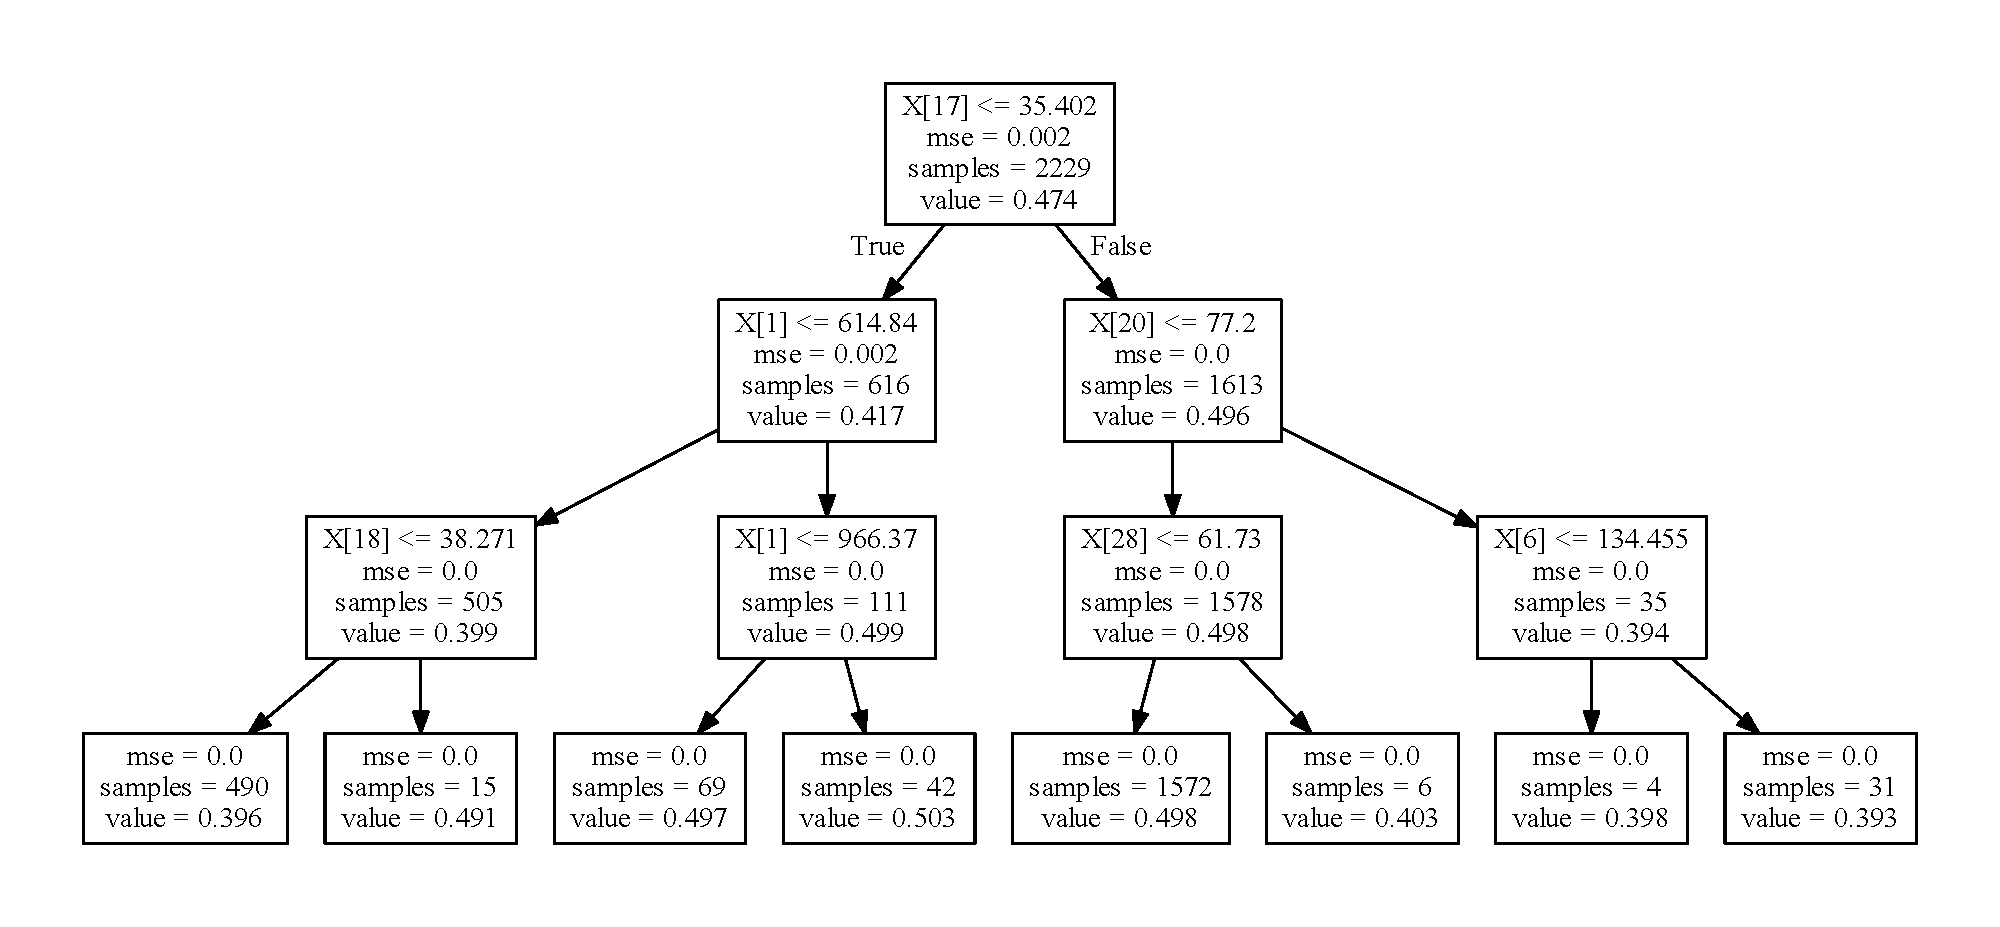
\includegraphics[width=\linewidth]{regression_tree_d3.pdf}
\end{solution}

\end{subtask}
\end{task}
